%Notes by Harsh Mistry 
%CS 444
%based on Template from : https://www.cs.cmu.edu/~ggordon/10725-F12/template.tex

\documentclass{article}
\setlength{\oddsidemargin}{0.25 in}
\setlength{\evensidemargin}{-0.25 in}
\setlength{\topmargin}{-0.6 in}
\setlength{\textwidth}{6.5 in}
\setlength{\textheight}{8.5 in}
\setlength{\headsep}{0.75 in}
\setlength{\parindent}{0 in}
\setlength{\parskip}{0.1 in}
\usepackage{amsfonts,graphicx, amssymb}
\usepackage[fleqn]{amsmath}
\usepackage{fixltx2e}
\usepackage{color}
\usepackage{tcolorbox}
\usepackage{lipsum}
\usepackage{listings}
\graphicspath{ {./images/} }
\usepackage{scrextend}
\tcbuselibrary{skins,breakable}
\usetikzlibrary{shadings,shadows}
\newcounter{lecnum}
\renewcommand{\thepage}{\thelecnum-\arabic{page}}
\renewcommand{\thesection}{\thelecnum.\arabic{section}}
\renewcommand{\theequation}{\thelecnum.\arabic{equation}}
\renewcommand{\thefigure}{\thelecnum.\arabic{figure}}
\renewcommand{\thetable}{\thelecnum.\arabic{table}}
\newcommand{\lecture}[4]{
   \pagestyle{myheadings}
   \thispagestyle{plain}
   \newpage
   \setcounter{lecnum}{#1}
   \setcounter{page}{1}
   
   
%Info Box 
   \begin{center}
   \framebox{
      \vbox{\vspace{2mm}
    \hbox to 6.28in { {\bf CS 444 - Compiler Construction 
	\hfill Winter 2020} }
       \vspace{4mm}
       \hbox to 6.28in { {\Large \hfill Lecture #1: #2  \hfill} }
       \vspace{2mm}
       \hbox to 6.28in { {\it Lecturer: #3 \hfill Notes By: #4} }
      \vspace{2mm}}
   }
   \end{center}
   
   \markboth{Lecture #1: #2}{Lecture #1: #2}



 
}

\renewcommand{\cite}[1]{[#1]}
\def\beginrefs{\begin{list}%
        {[\arabic{equation}]}{\usecounter{equation}
         \setlength{\leftmargin}{2.0truecm}\setlength{\labelsep}{0.4truecm}%
         \setlength{\labelwidth}{1.6truecm}}}
\def\endrefs{\end{list}}
\def\bibentry#1{\item[\hbox{[#1]}]}

\newcommand{\fig}[3]{
			\vspace{#2}
			\begin{center}
			Figure \thelecnum.#1:~#3
			\end{center}
	}
	
\newcommand{\pipe}{\(\mid\)}
\newcommand{\ctr}{\(\wedge\)}

\newtheorem{theorem}{Theorem}[lecnum]
\newtheorem{lemma}[theorem]{Lemma}
\newtheorem{ex}[theorem]{Example}
\newtheorem{proposition}[theorem]{Proposition}
\newtheorem{claim}[theorem]{Claim}
\newtheorem{corollary}[theorem]{Corollary}
\newtheorem{definition}[theorem]{Definition}
\newenvironment{proof}{{\bf Proof:}}{\hfill\rule{2mm}{2mm}}
\newcommand\E{\mathbb{E}}

%color definitions :
\definecolor{darkred}{rgb}{0.55, 0.0, 0.0}
\definecolor{lightcoral}{rgb}{0.94, 0.5, 0.5}
\definecolor{tomato}{rgb}{1.0, 0.39, 0.28}
\definecolor{lightgray}{rgb}{.9,.9,.9}
\definecolor{darkgray}{rgb}{.4,.4,.4}
\definecolor{purple}{rgb}{0.65, 0.12, 0.82}
\definecolor{lightgreen}{rgb}{0.56, 0.93, 0.56}
\definecolor{darkgreen}{rgb}{0.0, 0.2, 0.13}
\definecolor{limegreen}{rgb}{0.2, 0.8, 0.2}
\definecolor{lightblue}{rgb}{0.68, 0.85, 0.9}
\definecolor{darkblue}{rgb}{0.0, 0.0, 0.55}


%Environments
\newenvironment{exblock}[1]{%
    \tcolorbox[beamer,%
    noparskip,breakable,
    colback=lightgreen,colframe=darkgreen,%
    colbacklower=limegreen!75!lightgreen,%
    title=#1]}%
    {\endtcolorbox}

\newenvironment{ablock}[1]{%
    \tcolorbox[beamer,%
    noparskip,breakable,
    colback=lightcoral,colframe=darkred,%
    colbacklower=tomato!75!lightcoral,%
    title=#1]}%
    {\endtcolorbox}

\newenvironment{cblock}[1]{%
    \tcolorbox[beamer,%
    noparskip,breakable,
    colback=lightblue,colframe=darkblue,%
    colbacklower=darkblue!75!lightblue,%
    title=#1]}%
    {\endtcolorbox}


%Languages
\lstdefinelanguage{JavaScript}{
  keywords={typeof, new, true, false, catch, function, return, null, catch, switch, var, if, in,  fi, while, do, else, case, break},
  keywordstyle=\color{blue}\bfseries,
  ndkeywords={class, export, boolean, throw, implements, import, this},
  ndkeywordstyle=\color{darkgray}\bfseries,
  identifierstyle=\color{black},
  sensitive=false,
  comment=[l]{//},
  morecomment=[s]{/*}{*/},
  commentstyle=\color{purple}\ttfamily,
  stringstyle=\color{red}\ttfamily,
  morestring=[b]',
  morestring=[b]"
}

%Listings
\lstset{
   language=JavaScript,
   backgroundcolor=\color{lightgray},
   extendedchars=true,
   basicstyle=\footnotesize\ttfamily,
   showstringspaces=false,
   showspaces=false,
   numbers=left,
   numberstyle=\footnotesize,
   numbersep=9pt,
   tabsize=2,
   breaklines=true,
   showtabs=false,
   captionpos=b
}


%Start of Document 
\begin{document}

\lecture{2}{January 8th, 2020}{Ond\u{r}ej Lhot\'{a}k}{Harsh Mistry}

\section{Analysis}

\begin{itemize}
\item Answers two questions
\begin{itemize}
		\item Is the input valid?
		\item What does the program mean? 
\end{itemize}

\item Formal Languages
		\item Precise specs of sets of strings
\item Lexical analysis (Screening) (JLS Ch 3) 
\begin{itemize}
		\item Scanning is about spliting the input sequence of characters into a sequence of tokens
		\item Int main (int foo) {return foo;} 
		\begin{enumerate}
			\item Int 
			\item Main 
			\item (
			\item Int 
			\item  Foo 
			\item  )
			\item  {
			\item  Return
			\item  Foo 
			\item  ;
			\item 1 }
		\end{enumerate}
		
\end{itemize}

\item Creating a scanner
\begin{enumerate}
		\item. Just write some code
		\item. Maximal munch algorithm using a DFA
		\begin{enumerate}
			\item Design DFA by hand
			\item Use a tool. Pass a regular expressions into lex to get a DFA. 
			\begin{itemize}
			\item \(REGEX \rightarrow NFA \rightarrow DFA\)
			\end{itemize}
		\end{enumerate}

\end{enumerate}

\item Converting Regular Expressions to NFA

\begin{tabular}{|c|c||c|}
\hline 
$\epsilon$ & $meaning L(\epsilon)$ & NFA \\ 
\hline 
$\emptyset $ & \{\} & 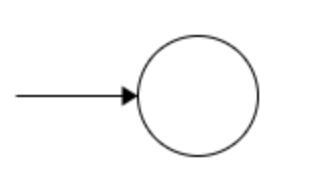
\includegraphics[scale=0.2]{3} \\ 
\hline 
$ a \in \sum $ & $\{a\} $ & 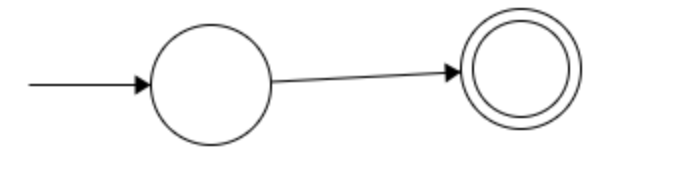
\includegraphics[scale=0.2]{1} \\ 
\hline 
$ \varepsilon $ &  $\{\varepsilon\}$ & 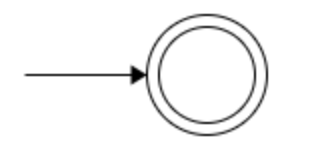
\includegraphics[scale=0.2]{2} \\ 
\hline 
$e_1 e_2$ & $\{x y |  x \in L(e_1), y \in L(e_2) \}$ & 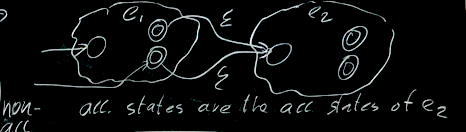
\includegraphics[scale=0.3]{4} \\ 
\hline 
$e_1 | e_2$ &  $L(e_1) \cup L(e_2) $ & 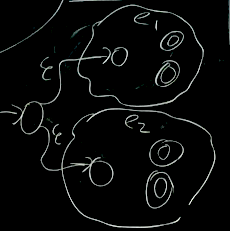
\includegraphics[scale=0.3]{5}  \\ 
\hline 
$e^* $ & $L(\varepsilon | e | ee | eee | \hdots )$ & 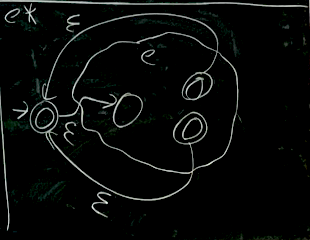
\includegraphics[scale=0.3]{6} \\ 
\hline
\end{tabular}
	

\end{itemize}

\end{document}







